\documentclass[12pt,a4paper]{report}
\usepackage[left=3.00cm, right=2.00cm, top=2.00cm, bottom=2.00cm]{geometry}
\usepackage{vntex}
\usepackage{listings}
\usepackage{amsmath}
\usepackage{amssymb}
\usepackage{graphicx}
\usepackage{tabularx}
\usepackage{colortbl}
\usepackage{hhline}
\newcommand{\shellcmd}[1]{\\\indent\indent\texttt{\footnotesize\# #1}\\}
\newcommand{\nocontentsline}[3]{}
\newcommand{\tocless}[2]{\bgroup\let\addcontentsline=\nocontentsline#1{#2}\egroup}
\author{DSH + NAT}
\usepackage{xcolor}
\usepackage{colortbl}
\usepackage{hhline}
\setcounter{secnumdepth}{5}
\definecolor{codegreen}{rgb}{0,0.6,0}
\definecolor{codegray}{rgb}{0.5,0.5,0.5}
\definecolor{codepurple}{rgb}{0.58,0,0.82}
\definecolor{backcolour}{rgb}{0.95,0.95,0.92}

\lstdefinestyle{mystyle}{
	backgroundcolor=\color{backcolour},   
	commentstyle=\color{codegreen},
	keywordstyle=\color{magenta},
	numberstyle=\tiny\color{codegray},
	stringstyle=\color{codepurple},
	basicstyle=\ttfamily\footnotesize,
	breakatwhitespace=false,         
	breaklines=true,                 
	captionpos=b,                    
	keepspaces=true,                 
	numbers=left,                    
	numbersep=5pt,                  
	showspaces=false,                
	showstringspaces=false,
	showtabs=false,                  
	tabsize=2
}

\lstset{style=mystyle}
\usepackage{tikz}
\usetikzlibrary{calc}
\title{Đề cương chi tiết Ver 1}

\begin{document}
	\begin{titlepage}
		\begin{tikzpicture}[remember picture,overlay,inner sep=0,outer sep=0]
			\draw[blue!70!black,line width=4pt] ([xshift=-1.5cm,yshift=-2cm]current page.north east) coordinate (A)--([xshift=1.5cm,yshift=-2cm]current page.north west) coordinate(B)--([xshift=1.5cm,yshift=2cm]current page.south west) coordinate (C)--([xshift=-1.5cm,yshift=2cm]current page.south east) coordinate(D)--cycle;
			
			\draw ([yshift=0.5cm,xshift=-0.5cm]A)-- ([yshift=0.5cm,xshift=0.5cm]B)--
			([yshift=-0.5cm,xshift=0.5cm]B) --([yshift=-0.5cm,xshift=-0.5cm]B)--([yshift=0.5cm,xshift=-0.5cm]C)--([yshift=0.5cm,xshift=0.5cm]C)--([yshift=-0.5cm,xshift=0.5cm]C)-- ([yshift=-0.5cm,xshift=-0.5cm]D)--([yshift=0.5cm,xshift=-0.5cm]D)--([yshift=0.5cm,xshift=0.5cm]D)--([yshift=-0.5cm,xshift=0.5cm]A)--([yshift=-0.5cm,xshift=-0.5cm]A)--([yshift=0.5cm,xshift=-0.5cm]A);
			
			
			\draw ([yshift=-0.3cm,xshift=0.3cm]A)-- ([yshift=-0.3cm,xshift=-0.3cm]B)--
			([yshift=0.3cm,xshift=-0.3cm]B) --([yshift=0.3cm,xshift=0.3cm]B)--([yshift=-0.3cm,xshift=0.3cm]C)--([yshift=-0.3cm,xshift=-0.3cm]C)--([yshift=0.3cm,xshift=-0.3cm]C)-- ([yshift=0.3cm,xshift=0.3cm]D)--([yshift=-0.3cm,xshift=0.3cm]D)--([yshift=-0.3cm,xshift=-0.3cm]D)--([yshift=0.3cm,xshift=-0.3cm]A)--([yshift=0.3cm,xshift=0.3cm]A)--([yshift=-0.3cm,xshift=0.3cm]A);
			
		\end{tikzpicture}
		\begin{center}
			BAN CƠ YẾU CHÍNH PHỦ\\
			\textbf{HỌC VIỆN KỸ THUẬT MẬT MÃ}
		\end{center}
		\begin{figure}[h]
			\centering
			\includegraphics[width=0.25\linewidth]{"Pics/Logo HV"}
			\label{fig:logo-hv}
		\end{figure}
		
		\begin{center}
			{\Huge ĐỀ CƯƠNG\\}
			{\large CHUYÊN ĐỀ AN TOÀN HỆ THỐNG THÔNG TIN\\}
			\textbf{Nghiên cứu giải pháp đảm bảo an toàn dữ liệu trên Kubernetes}
		\end{center}
		\bigskip
		\begin{flushright}
			\large{Ngành: An toàn thông tin}
		\end{flushright}
		\vspace{30mm}
		\begin{flushleft}
			\textit{Sinh viên thực hiện:}\\
			\textbf{Nguyễn Anh Tuấn}\\
			Mã sinh viên: AT160258\\
			\textbf{Đặng Sơn Hà}\\
			Mã sinh viên: AT160220
			\bigskip\\
			\textit{Người hướng dẫn:}\\
			\textbf{TS. Nguyễn Mạnh Thắng}\\
			Khoa An toàn thông tin - Học viện Kỹ thuật mật mã
		\end{flushleft}
		\vfill
		\begin{center}
			Hà Nội, 2022
		\end{center}
		
	\end{titlepage}
	
	\tableofcontents
	
	\chapter*{\centering Lời cảm ơn}
	\addcontentsline{toc}{chapter}{Lời cảm ơn}
	\hspace{1cm}Nhóm chúng em xin chân thành cảm ơn các thầy cô trường Học viện Kỹ thuật Mật mã nói chung, quý thầy cô của khoa An toàn thông tin nói riêng đã tận tình dạy bảo, truyền đạt kiến thức cho chúng em trong suốt quá trình học.\\
	
	\hspace{1cm} Kính gửi đến Thầy Nguyễn Mạnh Thắng lời cảm ơn chân thành và sâu sắc nhất, cảm ơn thầy đã tận tình theo sát, chỉ bảo và hướng dẫn cho nhóm em trong quá trình thực hiện đề tài này. Thầy không chỉ hướng dẫn chúng em những kiến thức chuyên ngành, mà còn giúp chúng em học thêm những kĩ năng mềm, tinh thần học hỏi, thái độ khi làm việc nhóm.\\
	
	\hspace{1cm}Trong quá trình tìm hiểu nhóm chúng em xin cảm ơn các bạn sinh viên đã góp ý, giúp đỡ và hỗ trợ nhóm em rất nhiều trong quá trình tìm hiểu và làm đề tài.\\
	
	\hspace{1cm}Do kiến thức còn nhiều hạn chế nên không thể tránh khỏi những thiếu sót trong quá trình làm đề tài.Chúng em rất mong nhận được sự đóng góp ý kiến của quý thầy cô để đề tài của chúng em đạt được kết quả tốt hơn.\\
	\bigskip \\
	\textbf{Chúng em xin chân thành cảm ơn!}
	\chapter*{\centering Lời mở đầu}
	\addcontentsline{toc}{chapter}{Lời mở đầu}
	\hspace{1cm}{Trong những năm gần đây, Kubernetes đã trở thành một trong những công cụ quản lý container phổ biến nhất. Điều này là do sự phát triển mạnh mẽ của Kubernetes, cũng như sự phổ biến của container. Trong các doanh nghiệp hiện nay, Kubernetes là một phần không thể thiếu được sử dụng để quản lý các ứng dụng container, cung cấp các dịch vụ như load balancing, autoscaling, logging, monitoring, backup và restore, cũng như quản lý các tài nguyên của các ứng dụng như CPU, Memory, Storage, Network. Tuy nhiên, việc sử dụng Kubernetes cũng có những hạn chế, đặc biệt là trong việc quản lý các cấu hình nhạy cảm của ứng dụng và các tài nguyên của ứng dụng. Vì vậy, trong đề tài này, chúng ta sẽ tìm hiểu về Vault, một công cụ quản lý secret phổ biến nhất hiện nay, được phát triển bởi HashiCorp. \\}
	
	{\hspace{0.3cm}Vault được sử dụng để quản lý các secret như username, password, token, key, certificate, API key, SSH key, license key, database connection và các thông tin khác. Vì vậy trong tương lai, Vault sẽ là một trong những công cụ quản lý secret không thể thiếu trong Kubernetes.\\}
	
	\hspace{0.3cm}Với những lí do trên, bài toán đặt ra ở đây là làm sao để triển khai Vault trên cụm Kubernetes. Vậy nên, đề tài “Nghiên cứu giải pháp đảm bảo an toàn dữ liệu trên K8S” được thực hiện trong báo cáo có ý nghĩa khoa học và mang tính thực tiễn cao.\\
	
	\chapter{Giới thiệu về Kurbenetes}
	\section{Tổng quan về Kurbenetes}
	
	\hspace{1cm}{Kubernetes hoặc k8s là một nền tảng mã nguồn mở giúp tự động hóa việc quản lý, mở rộng và triển khai ứng dụng dưới dạng container. Kubernetes còn được gọi là Container Orchestration Engine (hiểu nôm na là công cụ điều phối container). Kubernetes loại bỏ rất nhiều các quy trình thủ công liên quan đến việc triển khai và mở rộng các containerized applications. Các ứng dụng có thể khác nhau về kích thước: từ 1 cho đến hàng nghìn server. Với Kubernetes chúng ta có thể phát triển application một cách linh hoạt và đáng tin cậy. \\}
	
	\hspace{0.3cm}{Trách nhiệm chính của Kubernetes là container orchestration (dịch ra có nghĩa điều phối container). Kubernetes đảm bảo rằng tất cả container được lên lịch chạy trên các cụm server (cluster) (server ở đây có thể là physical machine hoặc virtual machine). Ngoài ra, Kubernetes còn có chức năng theo dõi hoạt động của từng container, mở rộng các containers và quản lý tình trạng của các containers theo thời gian. Khi một container nào đó gặp trục trặc, dừng hoạt động thì Kubernetes sẽ thay thế container đó. \\}
	
	\hspace{0.3cm}{Kubernetes ban đầu được các kỹ sư Google phát triển vào năm 2014. Và Google cũng là một trong những cái tên tiên phong đóng góp cho công cuộc phát triển công nghệ Linux container. \\}
	
	\hspace{0.3cm}{Kubernetes ban đầu được các kỹ sư Google phát triển vào năm 2014. Và Google cũng là một trong những cái tên tiên phong đóng góp cho công cuộc phát triển công nghệ Linux container. \\}
	
	\hspace{0.3cm}{Red Hat là một trong những công ty đầu tiên hợp tác với Google trong dự án Kubernetes trước khi Kubernetes được ra mắt, và trở thành nhà tài trợ lớn thứ 2 cho dự án ngay từ những ngày đầu. Và Google đã tặng lại dự án Kubernetes cho Cloud Native Computing Foundation (CNCF - thành lập năm 2015). Kubernetes đã trở thành một project của tổ chức này cho đến thời điểm hiện tại. Năm 2018, Kubernetes Project đạt vị trí thứ 9 về số lượt commit trên Github.}
	\subsection{Các thành phần trong kubernetes}
	
	\hspace{1cm}{Khi bạn triển khai Kubernetes, bạn sẽ nhận được một Cluster (cụm máy chủ). \\}
	
	\hspace{0.3cm}{Một Cluster Kubernetes bao gồm một tập hợp các máy worker, được gọi là Node, chạy các ứng dụng được đóng gói. Mỗi Cluster có ít nhất một Node. \\}
	
	\hspace{0.3cm}{(Các) Node lưu trữ các Pod - Một nhóm gồm một hoặc nhiều containers được triển khai cho single Node, nhóm này chia sẻ chung không gian lưu trữ, IP address, hostname, và những nguồn khác. \\}
	
	\hspace{0.3cm}{Các Control Plane quản lý các Node và các Pod trong Cluster. Trong môi trường production, Control Plane thường chạy trên nhiều máy tính và một Cluster thường chạy nhiều Node, mang lại khả năng chịu lỗi và tính sẵn sàng cao. \\}
	
	\hspace{0.3cm}{Trên đây là sơ đồ của một cụm Kubernetes với tất cả các thành phần được gắn với nhau.}
	
	\begin{figure}
		\centering
		\includegraphics[width=1\textwidth]{"Pics/components-of-kubernetes"}
		\caption{\label{fig:components-of-kubernetes} Sơ đồ của một cụm Kubernetes.}
		\label{fig:components-of-kubernetes}
	\end{figure}
	
	\subsubsection{Các thành phần Control Plane (Master)}
	
	\hspace{1cm}{Các thành phần Control Plane đưa ra các quyết định chung về Cluster (ví dụ: lập lịch), cũng như phát hiện và phản hồi các sự kiện của Cluster. \\}
	
	\hspace{0.3cm}{Các thành phần Control Plane có thể được chạy trên bất kỳ máy nào trong Cluster. Tuy nhiên, để đơn giản, thiết lập tập lệnh thường khởi động tất cả các thành phần Control Plane trên cùng một máy và không chạy các container của người dùng trên máy này. \\}
	
	\hspace{0.3cm}{Đối với cluster nhỏ , Master có thể chạy trên một Node, nhưng trong một cluster lớn, để đảm bảo tính khả dụng (trong tiếng anh là High-Availability) thì Master có thể được chạy trên nhiều Node. (Tính khả dụng có nghĩa là Khi mà một Node trong cluster dừng hoạt động thì hệ thống vẫn duy trì như không có gì xảy ra). Master sẽ bao gồm 5 thành phần chính sau:}
	
	\begin{itemize}
	\item \textbf{kube-apiserver:}
	\smallskip
	\subitem
	API Server là một thành phần của Control Plane. Đúng theo tên gọi, đây chính là server cung cấp REST API cho Kubernetes Cluster. Nó có nhiệm vụ đặt Pod vào Node, đồng bộ hoá thông tin của Pod bằng REST API tiếp nhận cài đặt, xác thực và thiết lập cho các objects pod/service/replicationController.
	
	\item \textbf{Etcd:}
	\smallskip
	\subitem
	Etcd là Kho lưu trữ giá trị khóa nhất quán và có tính khả dụng cao được sử dụng làm kho dự phòng để lưu trữ toàn bộ cấu hình, trạng thái và metadata của Kubernetes Cluster.
	\smallskip
	\subitem Trong các cluster nhỏ, Etcd có thể chạy trên cùng một Node với các thành phần khác. Nhưng trong các cluster lớn, Etcd có thể chạy dự phòng trên nhiều Node để đảm bảo tính khả dụng của toàn hệ thống. Nếu cụm Kubernetes của bạn sử dụng Etcd làm nơi lưu trữ sao lưu, hãy đảm bảo rằng bạn có kế hoạch sao lưu cho những dữ liệu đó.
	
	\item \textbf{kube-controller-manager:}
	\smallskip
	\subitem
	Kube Controller Manage một tập hợp các controller khác nhau để chạy các bộ điều khiển quy trình theo dõi các cập nhật trạng thái của Kubernetes Cluster thông qua API và thực hiện các thay đổi đối với Cluster sao cho phù hợp. 
	\smallskip
	\subitem Về mặt logic, mỗi bộ điều khiển là một quy trình riêng biệt, nhưng để giảm độ phức tạp, tất cả chúng đều được biên dịch thành một tệp nhị phân duy nhất và chạy trong một quy trình duy nhất.
	\smallskip
	\subitem Một số loại bộ điều khiển có thể kể đến:
	\begin{itemize}
		\item Node controller: Chịu trách nhiệm thông báo và phản hồi khi các Node gặp sự cố.

		
		\item \textbf{Etcd:}
		\subitem
		Etcd là Kho lưu trữ giá trị khóa nhất quán và có tính khả dụng cao được sử dụng làm kho dự phòng để lưu trữ toàn bộ cấu hình, trạng thái và metadata của Kubernetes Cluster.
		
		\hspace{0.8cm}{Trong các cluster nhỏ, Etcd có thể chạy trên cùng một Node với các thành phần khác. Nhưng trong các cluster lớn, Etcd có thể chạy dự phòng trên nhiều Node để đảm bảo tính khả dụng của toàn hệ thống. Nếu cụm Kubernetes của bạn sử dụng Etcd làm nơi lưu trữ sao lưu, hãy đảm bảo rằng bạn có kế hoạch sao lưu cho những dữ liệu đó.}
		

		\item Service Account \& Token controllers: Tạo tài khoản mặc định và mã thông báo truy cập API cho không gian tên mới.
	\end{itemize}

	\item \textbf{cloud-controller-manager:}
	\smallskip
	\subitem
	Là một tập hợp các logic dành riêng cho đám mây (GCP, AWS, Azure) cho phép bạn liên kết Kubernetes Cluster với API của nhà cung cấp đám mây và tách các thành phần tương tác với nền tảng đám mây đó khỏi các thành phần chỉ tương tác với cụm của bạn. Cloud-controller-manager chỉ chạy các bộ điều khiển dành riêng cho nhà cung cấp dịch vụ đám mây của bạn. Nếu bạn đang chạy Kubernetes tại cơ sở của riêng mình hoặc trong môi trường học tập bên trong PC của riêng bạn, cụm không có trình quản lý bộ điều khiển đám mây.
	\smallskip
	\subitem Cũng như với kube-controller-manager, cloud-controller-manager kết hợp một số vòng điều khiển độc lập về mặt logic thành một tệp nhị phân duy nhất mà bạn chạy như một quy trình duy nhất. Bạn có thể chia tỷ lệ theo chiều ngang (chạy nhiều hơn một bản sao) để cải thiện hiệu suất hoặc để giúp tăng khả năng chịu lỗi.
	\smallskip
	\subitem Các bộ điều khiển sau có thể có các phần phụ thuộc của nhà cung cấp dịch vụ đám mây:
	\begin{itemize}
	\item Node controller: Để kiểm tra nhà cung cấp đám mây để xác định xem một Node đã bị xóa trong đám mây sau khi nó ngừng phản hồi hay chưa.
	
	\item Route controller: Để thiết lập định tuyến trong cơ sở hạ tầng đám mây cơ bản.
	
	\item Service controller: Để tạo, cập nhật và xóa bộ cân bằng tải của nhà cung cấp dịch vụ đám mây.
	\end{itemize}
	
	\item \textbf{kube-scheduler:}
	\smallskip
	\subitem
	Sử dụng Kubernetes API để tìm, theo dõi các Pod chưa được lên lịch hoặc mới được tạo nhưng không được chỉ định Node. Sau đó, scheduler sẽ đặt các Pod này vào các Node dựa trên tài nguyên và các ràng buộc khác được định nghĩa trong manifest file của Pod. Scheduler sẽ cố gắng đảm bảo rằng các Pod của cùng một application sẽ được phân phối trên các Node khác nhau để đảm bảo tính khả dụng.
	\smallskip
	\subitem Các yếu tố được tính đến để đưa ra quyết định lập lịch bao gồm: yêu cầu tài nguyên cá nhân và tập thể, các ràng buộc về phần cứng / phần mềm / chính sách, thông số kỹ thuật về mối quan hệ và chống mối quan hệ, vị trí dữ liệu, can thiệp giữa khối lượng công việc và thời hạn.
	\end{itemize}


	\subsubsection{Các thành phần Worker}
	
	\hspace{1cm}{Có nhiệm vụ xử lý khối lượng công việc của application trong cluster, duy trì các nhóm đang chạy và cung cấp môi trường runtime cho Kubernetes. Worker sẽ bao gồm 3 thành phần chính sau:}
	\begin{itemize}
		\item \textbf{kubelet:}
		\smallskip
		\subitem
		Kubelet chạy trên mỗi Worker Node. Nó đảm bảo rằng các container đang chạy trong một Pod và có trách nhiệm giám sát giao tiếp với master node và quản lý các Pod. Kubelet sử dụng CRI (Container Runtime Interface - Giao diện thời gian chạy vùng chứa) để giao tiếp với container runtime trên cùng một Node đó. Kubelet không quản lý các vùng chứa không được tạo bởi Kubernetes.
		
		\item \textbf{kube-proxy:}
		\smallskip
		\subitem
		Là một proxy mạng chạy trên mỗi Node trong Cluster. Nó có trách nhiệm quản lý, duy trì các quy tắc mạng trên mỗi Node. Các quy tắc mạng này cho phép giao tiếp mạng với Pod của bạn từ các phiên mạng bên trong hoặc bên ngoài Cluster. kube-proxy sử dụng lớp lọc gói của hệ điều hành nếu có và nó có sẵn. Nếu không, kube-proxy sẽ tự chuyển tiếp lưu lượng.
		
		\item \textbf{Container Runtime:}
		\smallskip
		\subitem
		Là phần mềm chịu trách nhiệm chạy các container. Kubernetes hỗ trợ một số container runtime như: Docker, containerd, CRI-O và bất kỳ triển khai nào của Kubernetes CRI (Container Runtime Interface).
	\end{itemize}
	
	\section{Kiến trúc của cụm}
	
	\subsection{Node}
	
		\hspace{1cm}{Kubernetes chạy khối lượng công việc bằng cách đặt các container vào các Pod để chạy trên các Node. Một Node có thể là một máy ảo hoặc vật lý, tùy thuộc vào cụm. Mỗi Node được quản lý bởi control plane và chứa các dịch vụ cần thiết để chạy các Pod.\\}
	
	\hspace{0.3cm}{Thông thường, có một số Node trong một cụm; trong môi trường học tập hoặc tài nguyên hạn chế, có thể chỉ có một Node.\\}
	
	\hspace{0.3cm}{Các thành phần trên một Node bao gồm kubelet, container runtime (là thành phần giúp chạy các ứng dụng dưới dạng container), và kube-proxy.}
	
	\begin{figure}[h]
		\centering
		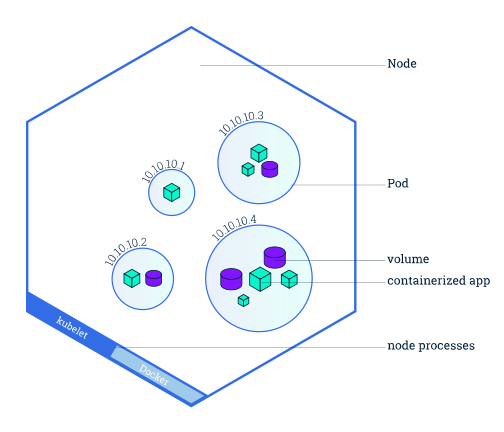
\includegraphics[width=0.7\linewidth]{Pics/nodes}
		\caption{\label{fig:nodes} Cấu tạo của Nodes.}
		\label{fig:nodes}
	\end{figure}
	
	\subsubsection{Quản lý}
	
	\hspace{1cm}{Có hai cách chính để thêm các Node vào máy chủ API:}
	
	\begin{enumerate}
		\item Kubelet trên một Node tự đăng ký vào control plane
		\item Thêm một đối tượng Node theo cách thủ công\\
	\end{enumerate}
	
	\hspace{0.3cm}{Sau khi bạn tạo một đối tượng Node hoặc kubelet trên Node tự đăng ký, control plane sẽ kiểm tra xem đối tượng Node mới có hợp lệ hay không. Ví dụ: nếu bạn cố gắng tạo một Node từ tệp kê khai JSON sau:\\}
	
	\begin{lstlisting}[language=Bash]
		{
			"kind": "Node",
			"apiVersion": "v1",
			"metadata": {
				"name": "10.240.79.157",
				"labels": {
					"name": "my-first-k8s-node"
				}
			}
		}
	\end{lstlisting}
	\smallskip
	
	\hspace{0.3cm}{Kubernetes tạo một đối tượng Node nội bộ. Kubernetes kiểm tra xem kubelet đã đăng ký với máy chủ API khớp với trường \texttt{metadata.name} của ứng dụng Node. Nếu Node hoạt động tốt (tức là tất cả các dịch vụ cần thiết đang chạy), thì Node đó đủ điều kiện để chạy Pod. Nếu không, Node đó sẽ bị bỏ qua đối với mọi hoạt động của cụm cho đến khi nó hoạt động bình thường.\\}
	
	\hspace{0.3cm}{Tên của một đối tượng Node phải là một tên miền phụ DNS hợp lệ.}
	
	\begin{itemize}
		\item \textbf{Tính duy nhất của tên Node}
		\smallskip
		\subitem Tên xác định một Node. Hai Node không thể có cùng tên cùng một lúc. Kubernetes cũng giả định rằng một tài nguyên có cùng tên là cùng một đối tượng. Trong trường hợp một Node, người ta mặc nhiên cho rằng một thể hiện sử dụng cùng tên sẽ có cùng trạng thái (ví dụ: cài đặt mạng, nội dung đĩa gốc) và các thuộc tính như nhãn Node. Điều này có thể dẫn đến sự không nhất quán nếu một phiên bản được sửa đổi mà không thay đổi tên của nó. Nếu Node cần được thay thế hoặc cập nhật đáng kể, đối tượng Node hiện có cần được xóa khỏi máy chủ API trước và thêm lại sau khi cập nhật.
		\smallskip
		\item \textbf{Tự đăng ký Node}
		\smallskip
		\subitem Khi cờ kubelet \texttt{--register-node} là \texttt{true} (mặc định), kubelet sẽ cố gắng tự đăng ký với máy chủ API. Đây là mẫu ưa thích, được sử dụng bởi hầu hết các bản phân phối.
		\smallskip
		\subitem Để tự đăng ký, kubelet được bắt đầu với các tùy chọn sau:
		
		\begin{itemize}
			\item \texttt{-kubeconfig} Đường dẫn đến thông tin đăng nhập để tự xác thực với máy chủ API.
			\item \texttt{-cloud-provider} Nói chuyện với một nhà cung cấp đám mây để đọc siêu dữ liệu về chính nó.
			\item \texttt{-register-node} Tự động đăng ký với máy chủ API.
			\item \texttt{-register-with-taints} Đăng ký Node với danh sách Taints đã cho (phân cách bằng dấu phẩy \texttt{<key>=<value>:<effect>}).
			
			No-op nếu \texttt{register-node} là sai.
			
			\item \texttt{-node-ip} Địa chỉ IP của Node.
			\item \texttt{-node-labels} - nhãn để thêm khi đăng ký Node trong cụm.
			\item \texttt{-node-status-update-frequency} Chỉ định tần suất kubelet đăng trạng thái Node của nó lên máy chủ API.
		\end{itemize}
		\smallskip
		\item \textbf{Quản lý Node thủ công}
		\smallskip
		\subitem Có thể tạo và sửa đổi các đối tượng Node bằng cách sử dụng kubectl.
		\smallskip
		\subitem Khi muốn tạo các đối tượng Node theo cách thủ công, hãy đặt cờ kubelet     \texttt{--register-node=false}.
		\smallskip
		\subitem Có thể sửa đổi các đối tượng Node bất kể cài đặt của \texttt{--register-node}. Ví dụ: bạn có thể đặt nhãn trên một Node hiện có hoặc đánh dấu Node đó là không thể lập lịch trình.
		\smallskip
		\subitem Có thể sử dụng nhãn trên Node kết hợp với bộ chọn Node trên Pod để kiểm soát việc lên lịch. Ví dụ: bạn có thể hạn chế một Pod chỉ đủ điều kiện chạy trên một tập hợp con các Nod có sẵn.
		\smallskip
		\subitem Việc đánh dấu một Node là không thể lập lịch trình sẽ ngăn bộ lập lịch đặt các Pod mới vào Node đó nhưng không ảnh hưởng đến các Pod hiện có trên Node. Điều này hữu ích như một bước chuẩn bị trước khi khởi động lại Node hoặc bảo trì khác.
		\subitem Để đánh dấu một Node không thể lên lịch, hãy chạy:\\
		\shellcmd{kubectl cordon \$NODENAME}
	\end{itemize}
	\subsubsection{Trạng thái Node}
	
	\hspace{1cm}{Trạng thái của Node chứa các thông tin sau:}
	\begin{enumerate}
		\item Địa chỉ
		\item Các điều kiện
		\item Năng lực và phân bổ
		\item Thông tin
	\end{enumerate}
	\smallskip
	\hspace{1cm}{Bạn có thể sử dụng \texttt{kubectl} để xem trạng thái của Node và các chi tiết khác.}
	
	\begin{itemize}
		\item \textbf{Địa chỉ}
		\smallskip
		\subitem Việc sử dụng các trường này khác nhau tùy thuộc vào nhà cung cấp dịch vụ đám mây hoặc cấu hình bare-metal.
		\begin{itemize}
			\item Tên máy chủ: Tên máy chủ được báo cáo bởi nhân của Node. Có thể được ghi đè thông qua tham số kubelet \texttt{-hostname-override}.
			\item IP bên ngoài: Điển hình là địa chỉ IP của Node có thể định tuyến bên ngoài (có sẵn từ bên ngoài cụm).
			\item InternalIP: Thông thường, địa chỉ IP của Node chỉ có thể định tuyến được trong cụm.
		\end{itemize}
		\smallskip
		\item \textbf{Các điều kiện}
		\smallskip
		\subitem Trường \texttt{conditions} mô tả trạng thái của tất cả các Node \texttt{Running}. Ví dụ về các điều kiện bao gồm:
		\begin{figure}
			\centering
			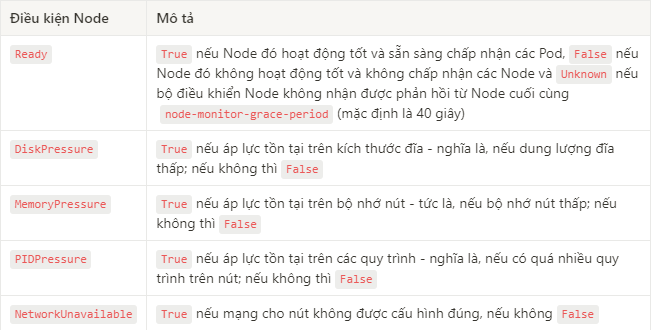
\includegraphics[width=1\linewidth]{Pics/conditions}
			\caption{\label{fig:conditions}Ví dụ về các điều kiện}
			\label{fig:conditions}
		\end{figure}
		\smallskip
		\subitem Trong API Kubernetes, điều kiện của Node được biểu diễn như một phần của \texttt{.status} của tài nguyên Node. Ví dụ: cấu trúc JSON sau đây mô tả một Node hoạt động tốt:
		\smallskip
		\begin{lstlisting}[language=Bash]
			"conditions": [
			{
				"type": "Ready",
				"status": "True",
				"reason": "KubeletReady",
				"message": "kubelet is posting ready status",
				"lastHeartbeatTime": "2019-06-05T18:38:35Z",
				"lastTransitionTime": "2019-06-05T11:41:27Z"
			}
			]
		\end{lstlisting}
		\smallskip
		\subitem Nếu \texttt{status} của Readly vẫn còn tình trạng \texttt{Unknown} hoặc \texttt{False} lâu hơn pod-eviction-timeout (một đối số được chuyển đến kube-controller-manager), thì bộ điều khiển Node sẽ kích hoạt quá trình do khởi tạo API trục xuất cho tất cả các Pod được gán cho Node đó. Thời gian chờ trục xuất mặc định là năm phút. Trong một số trường hợp khi không thể truy cập Node, máy chủ API không thể giao tiếp với kubelet trên Node. Quyết định xóa các Pod không thể được thông báo tới kubelet cho đến khi giao tiếp với máy chủ API được thiết lập lại. Trong thời gian chờ đợi, các Pod được lên lịch xóa có thể tiếp tục chạy trên Node được phân vùng.
		\smallskip
		\subitem Bộ điều khiển nút không buộc xóa các Pod cho đến khi được xác nhận rằng chúng đã ngừng chạy trong cụm. Có thể thấy các Nhóm có thể đang chạy trên một Node không thể truy cập được ở trạng thái \texttt{Terminating} hoặc \texttt{Unknown}. Trong trường hợp Kubernetes không thể suy luận từ cơ sở hạ tầng cơ bản nếu một Node đã rời khỏi cụm vĩnh viễn, quản trị viên cụm có thể cần phải xóa đối tượng Node bằng tay. Việc xóa đối tượng Node khỏi Kubernetes sẽ khiến tất cả các đối tượng Pod đang chạy trên Node bị xóa khỏi máy chủ API và giải phóng tên của chúng.
		\smallskip
		\subitem Khi xảy ra sự cố trên các Node, mặt phẳng điều khiển Kubernetes sẽ tự động tạo các dấu vết phù hợp với các điều kiện ảnh hưởng đến Node. Bộ lập lịch xem xét các yếu tố của Node khi gán một Pod cho một Node. Các Pod cũng có thể có dung sai cho phép chúng chạy trên một Node mặc dù nó có một taint cụ thể.
		\smallskip
		\item \textbf{Năng lực và phân bổ}
		\smallskip
		\subitem Mô tả các tài nguyên có sẵn trên Node: CPU, bộ nhớ và số lượng Pod tối đa có thể được lên lịch trên Node.
		\smallskip
		\subitem Các trường trong khối dung lượng cho biết tổng lượng tài nguyên mà một Node có. Khối có thể phân bổ cho biết lượng tài nguyên trên một Node có sẵn để các Pod thông thường sử dụng.
		\smallskip
		\item \textbf{Thông tin}
		\smallskip
		\subitem Mô tả thông tin chung về Node, chẳng hạn như phiên bản kernel, phiên bản Kubernetes (phiên bản kubelet và kube-proxy), chi tiết container runtime và hệ điều hành mà Node sử dụng. Kubelet thu thập thông tin này từ Node và xuất bản nó vào API Kubernetes.
	\end{itemize}
	
	\subsubsection{Heartbeats}
	
	\hspace{1cm}{Heartbeats, được gửi bởi các Node Kubernetes, giúp cụm xác định tính khả dụng của từng Node và thực hiện hành động khi phát hiện lỗi.\\}
	
	\hspace{0.3cm}{Đối với các Node có hai dạng Heartbeats:}
	\begin{itemize}
		\item cập nhật cho \texttt{.status} của một Node.
		\item Lease: Cho các đối tượng Node mượn trong không gian tên \texttt{kube-node-lease}. Mỗi Node có một đối tượng cho mượn được liên kết.
	\end{itemize}
	\hspace{0.3cm}{So với các bản cập nhật \texttt{.status} của Node, Lease là một tài nguyên nhẹ. Sử dụng Lease cho Heartbeats làm giảm tác động hiệu suất của các bản cập nhật này cho các cụm lớn.\\}
	
	\hspace{0.3cm}{Kubelet chịu trách nhiệm tạo và cập nhật các \texttt{.status} Node cũng như cập nhật các Lease liên quan của chúng.}
	
	\begin{itemize}
		\item Kubelet cập nhật \texttt{.status} của Node khi có thay đổi về trạng thái hoặc nếu không có bản cập nhật nào trong khoảng thời gian đã định cấu hình. Khoảng thời gian mặc định để cập nhật các Node là 5 phút, lâu hơn nhiều so với thời gian chờ mặc định 40 giây cho các Node không thể truy cập.
		\item Kubelet tạo và sau đó cập nhật đối tượng Lease của nó cứ sau 10 giây (khoảng thời gian cập nhật mặc định). Các bản cập nhật Lease xảy ra độc lập với các bản cập nhật cho \texttt{.status} của Node. Nếu cập nhật Lease không thành công, kubelet sẽ thử lại, sử dụng tính năng dự phòng theo cấp số nhân bắt đầu ở 200 mili giây và giới hạn ở 7 giây.
	\end{itemize}
	\subsubsection{Bộ điều khiển Node}
	
	\hspace{1cm}{Bộ điều khiển Node là một thành phần control plane Kubernetes quản lý các khía cạnh khác nhau của các Node.\\}
	
	\hspace{0.3cm}{Bộ điều khiển Node có nhiều vai trò trong vòng đời của Node. Đầu tiên là gán một khối CIDR cho Node khi nó được đăng ký (nếu chức năng gán CIDR được bật).\\}
	
	\hspace{0.3cm}{Thứ hai là giữ cho danh sách các Node nội bộ của bộ điều khiển Node được cập nhật với danh sách các máy có sẵn của nhà cung cấp đám mây. Khi chạy trong môi trường đám mây và bất cứ khi nào một Node không hoạt động tốt, bộ điều khiển Node sẽ hỏi nhà cung cấp đám mây xem VM cho Node đó có còn khả dụng hay không. Nếu không, bộ điều khiển Node sẽ xóa Node đó khỏi danh sách các Node của nó.\\}
	
	\hspace{0.3cm}{	Thứ ba là theo dõi tình trạng của các Node. Bộ điều khiển Node chịu trách nhiệm:}
	
	\begin{itemize}
		\item Trong trường hợp một Node không thể truy cập được, hãy cập nhật điều kiện trong trường \texttt{Ready} của \texttt{.status} Node. Trong trường hợp này, bộ điều khiển Node đặt điều kiện thành \texttt{Unknown}.
		\item Nếu một nút vẫn không thể truy cập: kích hoạt khởi tạo API trục xuất cho tất cả các Pod trên Node không thể truy cập. Theo mặc định, bộ điều khiển Node đợi 5 phút kể từ khi đánh dấu Node là \texttt{Unknown} và gửi yêu cầu trục xuất đầu tiên.
	\end{itemize}
	
	\hspace{0.3cm}{Theo mặc định, bộ điều khiển Node sẽ kiểm tra trạng thái của từng Node sau mỗi 5 giây. Khoảng thời gian này có thể được cấu hình bằng cách sử dụng cờ \texttt{--node-monitor-period} trên thành phần \texttt{kube-controller-manager}.}
	
	\subsection{Giao tiếp giữa các Node và Control Plane}
	
	\hspace{1cm}{Các giao tiếp bao gồm các đường dẫn giao tiếp giữa máy chủ API và cụm Kubernetes. Mục đích là cho phép người dùng tùy chỉnh cài đặt của họ để củng cố cấu hình mạng sao cho cụm có thể chạy trên mạng không đáng tin cậy (hoặc trên các IP công khai hoàn toàn trên nhà cung cấp dịch vụ đám mây).}
	
	\subsubsection{Node tới Control Plane}
	
	\hspace{1cm}{Kubernetes có mẫu API "hub-and-spoke". Tất cả việc sử dụng API từ các Node (hoặc Pod mà chúng chạy) sẽ chấm dứt tại máy chủ API. Không có thành phần Control plane nào khác được thiết kế để hiển thị các dịch vụ từ xa. Máy chủ API được định cấu hình để lắng nghe các kết nối từ xa trên cổng HTTPS an toàn (thường là 443) có bật một hoặc nhiều hình thức xác thực ứng dụng khách . Một hoặc nhiều hình thức ủy quyền phải được bật, đặc biệt nếu các yêu cầu ẩn danh hoặc mã thông báo tài khoản dịch vụ được cho phép.\\}
	
	\hspace{0.3cm}{Các Node phải được cung cấp chứng chỉ gốc công khai cho cụm sao cho chúng có thể kết nối an toàn với máy chủ API cùng với thông tin đăng nhập hợp lệ của ứng dụng khách. Một cách tiếp cận tốt là thông tin xác thực ứng dụng khách được cung cấp cho kubelet ở dạng chứng chỉ ứng dụng khách.\\}
	
	\hspace{0.3cm}{Các Pod muốn kết nối với máy chủ API có thể thực hiện việc này một cách an toàn bằng cách tận dụng tài khoản dịch vụ để Kubernetes sẽ tự động thêm chứng chỉ gốc công khai và mã thông báo hợp lệ vào nhóm khi nó được khởi tạo. Dịch vụ \texttt{kubernetes} (trong không gian tên \texttt{default}) được định cấu hình với một địa chỉ IP ảo được chuyển hướng (thông qua \texttt{kube-proxy}) đến điểm cuối HTTPS trên máy chủ API.\\}
	
	\hspace{0.3cm}{Các thành phần của control plane cũng giao tiếp với máy chủ API qua cổng an toàn.\\}
	
	\hspace{0.3cm}{Do đó, chế độ hoạt động mặc định cho các kết nối từ các Node và Pod chạy trên các Node đến Control plane được bảo mật theo mặc định và có thể chạy trên các mạng công cộng và/hoặc không đáng tin cậy.}
	
	\subsubsection{Control plane tới node}
	
	\hspace{1cm}{Có hai đường dẫn giao tiếp chính từ Control plane (máy chủ API) đến các Node. Đầu tiên là từ máy chủ API đến quy trình kubelet chạy trên mỗi Node trong cụm. Thứ hai là từ máy chủ API đến bất kỳ Node, Pod hoặc Service nào thông qua chức năng proxy của máy chủ API.}
	
	\begin{itemize}
		\item \textbf{API server đến kubelet}
		\smallskip
		\subitem Các kết nối từ máy chủ API đến kubelet được sử dụng cho:
		\begin{itemize}
			\item Tìm nạp nhật ký cho Pod.
			\item Đính kèm (thường thông qua \texttt{kubectl}) vào các Pod đang chạy.
			\item Cung cấp chức năng chuyển tiếp cổng của kubelet.
		\end{itemize}
		\subitem Các kết nối này kết thúc tại điểm cuối HTTPS của kubelet. Theo mặc định, máy chủ API không xác minh chứng chỉ phục vụ của kubelet, điều này làm cho kết nối phải chịu các cuộc tấn công trung gian và không an toàn khi chạy trên các mạng công cộng và/hoặc không đáng tin cậy.
		\smallskip
		\subitem Để xác minh kết nối này, hãy sử dụng cờ \texttt{--kubelet-certificate-authority} để cung cấp cho máy chủ API gói chứng chỉ gốc nhằm sử dụng để xác minh chứng chỉ cung cấp của kubelet.
		\smallskip
		\subitem Nếu không thể, hãy sử dụng đường hầm SSH giữa máy chủ API và kubelet nếu cần để tránh kết nối qua mạng công cộng hoặc không đáng tin cậy.
		\smallskip
		\subitem Cuối cùng, xác thực và/hoặc ủy quyền Kubelet phải được bật để bảo mật API kubelet.
		
		\item \textbf{API server đến các Node, Pod hoặc Service}
		\smallskip
		\subitem Các kết nối từ máy chủ API đến một Node, Pod hoặc Service mặc định là kết nối HTTP đơn giản và do đó không được xác thực cũng như không được mã hóa. Chúng có thể được chạy qua kết nối HTTPS an toàn bằng cách thêm tiền tố \texttt{https:} vào tên Node, Pod hoặc Service trong URL API, nhưng chúng sẽ không xác thực chứng chỉ do điểm cuối HTTPS cung cấp cũng như không cung cấp thông tin đăng nhập của khách hàng. Vì vậy, mặc dù kết nối sẽ được mã hóa nhưng nó sẽ không cung cấp bất kỳ đảm bảo nào về tính toàn vẹn. Các kết nối này hiện không an toàn để chạy qua các mạng công cộng hoặc không đáng tin cậy.
		
		\item \textbf{SSH tunnels}
		\smallskip
		\subitem Kubernetes hỗ trợ các SSH tunnel để bảo vệ các đường dẫn giao tiếp của control plane đến Node. Trong cấu hình này, máy chủ API khởi tạo một SSH tunnel tới từng Node trong cụm (kết nối với máy chủ SSH đang nghe trên cổng 22) và chuyển tất cả lưu lượng dành cho kubelet, Node, Pod hoặc Service qua tunnel. Tunnel này đảm bảo rằng lưu lượng không bị lộ ra bên ngoài mạng mà các Node đang chạy.
		\smallskip
		\subitem \textbf{Lưu ý}: SSH tunnel hiện không được dùng nữa, vì vậy không nên chọn sử dụng chúng trừ khi biết bản thân đang sử dụng với mục đích gì. Dịch vụ Konnectivity là sự thay thế cho kênh liên lạc này.
		
		\item \textbf{Dịch vụ Konnectivity}
		\smallskip
		\subitem Để thay thế cho các SSH tunnel, dịch vụ Konnectivity cung cấp proxy cấp TCP cho mặt phẳng điều khiển để liên lạc theo cụm. Dịch vụ Konnectivity bao gồm hai phần: máy chủ Konnectivity trong mạng control plane và tác nhân Konnectivity trong mạng Node. Tác nhân Konnectivity khởi tạo kết nối đến máy chủ Konnectivity và duy trì kết nối mạng. Sau khi kích hoạt dịch vụ Konnectivity, tất cả lưu lượng truy cập từ control plane đến các Node đều đi qua các kết nối này.
	\end{itemize}

	\subsection{Controllers}
	
	\hspace{1cm}{Trong chế tạo rô-bốt và tự động hóa, vòng lặp điều khiển là một vòng lặp không kết thúc điều chỉnh trạng thái của hệ thống.\\}
	
	\hspace{0.3cm}{Trong Kubernetes, bộ điều khiển là các vòng điều khiển theo dõi trạng thái trong cụm, sau đó thực hiện hoặc yêu cầu thay đổi nếu cần. Mỗi bộ điều khiển cố gắng di chuyển trạng thái cụm hiện tại đến gần trạng thái mong muốn hơn.}
	
	\subsubsection{Kiểu điều khiển}
	
	\hspace{1cm}{Bộ điều khiển theo dõi ít nhất một loại tài nguyên Kubernetes. Các đối tượng này có một trường thông số đại diện cho trạng thái mong muốn. (Các) bộ điều khiển cho tài nguyên đó chịu trách nhiệm làm cho trạng thái hiện tại tiến gần hơn đến trạng thái mong muốn đó.\\}
	
	\hspace{0.3cm}{Bộ điều khiển có thể tự thực hiện hành động; thông thường hơn, trong Kubernetes, bộ điều khiển sẽ gửi tin nhắn đến máy chủ API có tác dụng phụ hữu ích.}
	
	\begin{itemize}
		\item \textbf{Điều khiển thông qua máy chủ API}
		\smallskip
		\subitem Công việc của bộ điều khiển là một ví dụ về bộ điều khiển tích hợp Kubernetes. Bộ điều khiển tích hợp quản lý trạng thái bằng cách tương tác với máy chủ API cụm.
		\smallskip
		\subitem Công việc là một tài nguyên Kubernetes chạy một Pod, hoặc có thể là một số Pod, để thực hiện một tác vụ rồi dừng lại.
		\smallskip
		\subitem (Sau khi được lên lịch , các đối tượng Pod trở thành một phần của trạng thái mong muốn cho một kubelet).
		\smallskip
		\subitem Khi bộ điều khiển Công việc nhìn thấy một tác vụ mới, nó đảm bảo rằng, ở đâu đó trong cụm của bạn, các kubelet trên một nhóm các Node đang chạy đúng số lượng Pod để hoàn thành công việc. Bộ điều khiển công việc không tự chạy bất kỳ các Pod hoặc Container nào. Thay vào đó, bộ điều khiển Công việc yêu cầu máy chủ API tạo hoặc xóa Pod. Các thành phần khác trong control plane hành động dựa trên thông tin mới (có các Pod mới để lên lịch và chạy), và cuối cùng công việc đã hoàn thành.
		\smallskip
		\subitem Sau khi bạn tạo một Công việc mới, trạng thái mong muốn là Công việc đó đã được hoàn thành. Bộ điều khiển Công việc làm cho trạng thái hiện tại của Công việc đó gần với trạng thái mong muốn hơn: tạo các Pod thực hiện làm việc cho Công việc đó, để Công việc gần hoàn thành hơn.
		\smallskip
		\subitem Bộ điều khiển cũng cập nhật các đối tượng cấu hình chúng. Ví dụ: sau khi hoàn thành việc làm cho một Công việc, bộ điều khiển Công việc sẽ cập nhật đối tượng Công việc đó để đánh dấu nó \texttt{Finished}.
		
		\item \textbf{Điều khiển trực tiếp}
		\smallskip
		\subitem Ngược lại với Công việc, một số bộ điều khiển cần thực hiện thay đổi đối với những thứ bên ngoài cụm.
		\smallskip
		\subitem Các bộ điều khiển tương tác với trạng thái bên ngoài sẽ tìm thấy trạng thái mong muốn của chúng từ máy chủ API, sau đó giao tiếp trực tiếp với hệ thống bên ngoài để đưa trạng thái hiện tại đến gần trạng thái mong muốn hơn.
		\smallskip
		\subitem Điểm quan trọng ở đây là bộ điều khiển thực hiện một số thay đổi để mang lại trạng thái mong muốn, sau đó báo cáo trạng thái hiện tại trở lại máy chủ API của cụm. Các vòng điều khiển khác có thể quan sát dữ liệu được báo cáo đó và thực hiện các hành động của riêng chúng.
		\smallskip
		\subitem Với các cụm Kubernetes, control plane hoạt động gián tiếp với các công cụ quản lý địa chỉ IP, dịch vụ lưu trữ, API của nhà cung cấp đám mây và các dịch vụ khác bằng cách mở rộng Kubernetes để triển khai điều đó.
	\end{itemize}
	\subsubsection{Mong muốn so với trạng thái hiện tại}
	
	\hspace{1cm}{Kubernetes có chế độ xem hệ thống dựa trên đám mây và có thể xử lý thay đổi liên tục.\\}
	
	\hspace{0.3cm}{Cụm của bạn có thể thay đổi bất kỳ lúc nào khi công việc diễn ra và các vòng lặp điều khiển sẽ tự động khắc phục lỗi. Điều này có nghĩa là, có khả năng, cụm của bạn không bao giờ đạt đến trạng thái ổn định.\\}
	
	\hspace{0.3cm}{Miễn là các bộ điều khiển cho cụm đang chạy và có thể thực hiện các thay đổi hữu ích, nó không quan trọng nếu trạng thái tổng thể là ổn định hay không.}
	
	\subsubsection{Thiết kế}
	
	\hspace{1cm}{Như một nguyên lý trong thiết kế của nó, Kubernetes sử dụng rất nhiều bộ điều khiển mà mỗi bộ điều khiển quản lý một khía cạnh cụ thể của trạng thái cụm. Thông thường nhất, một vòng lặp điều khiển cụ thể (bộ điều khiển) sử dụng một loại tài nguyên làm trạng thái mong muốn của nó và có một loại tài nguyên khác mà nó quản lý để thực hiện trạng thái mong muốn đó. Ví dụ: bộ điều khiển cho Công việc theo dõi các đối tượng Công việc (để khám phá công việc mới) và các đối tượng Pod (để chạy Công việc, sau đó để xem khi nào công việc kết thúc). Trong trường hợp này, một cái gì đó khác tạo ra Công việc, trong khi bộ điều khiển Công việc tạo ra các Pod.\\}
	
	\hspace{0.3cm}{Thật hữu ích khi có các bộ điều khiển đơn giản thay vì một bộ vòng điều khiển nguyên khối được liên kết với nhau. Bộ điều khiển có thể bị lỗi, vì vậy Kubernetes được thiết kế để cho phép điều đó xảy ra.\\}
	
	\hspace{0.3cm}{\textbf{Ví dụ}: bạn có thể có các Deployment và Công việc; cả hai đều tạo ra các Pod. Bộ điều khiển công việc không xóa các Pod mà Deployment của bạn đã tạo, vì có thông tin (nhãn) bộ điều khiển có thể sử dụng để phân biệt các Pod đó.}
	
	\subsubsection{Các cách chạy bộ điều khiển}
	
	\hspace{1cm}{Kubernetes đi kèm với một bộ điều khiển tích hợp chạy bên trong kube-controller-manager. Các bộ điều khiển tích hợp này cung cấp các hành vi cốt lõi quan trọng.\\}
	
	\hspace{0.3cm}{Bộ điều khiển Deployment và Bộ điều khiển công việc là những ví dụ về bộ điều khiển là một phần của chính Kubernetes (bộ điều khiển "tích hợp"). Kubernetes cho phép bạn chạy một control plane có khả năng đối phó để nếu bất kỳ bộ điều khiển tích hợp nào bị lỗi, một phần khác của control plane sẽ đảm nhận công việc.\\}
	
	\hspace{0.3cm}{Bạn có thể tìm các bộ điều khiển chạy bên ngoài control plane để mở rộng Kubernetes. Hoặc, nếu muốn, bạn có thể tự viết một bộ điều khiển mới. Bạn có thể chạy bộ điều khiển của riêng mình dưới dạng một bộ Pod hoặc bên ngoài Kubernetes. Những gì phù hợp nhất sẽ phụ thuộc vào chức năng của bộ điều khiển cụ thể đó.}
	
	\section{Tổng quan về microservice}
	\hspace{1.0cm} {Microservices không còn là một điều mới lạ. Chúng ta đang thấy vi mô quy mô lớn triển khai dịch vụ với hàng ngàn dịch vụ. Nhưng cho dù có một hoặc hai dịch vụ hay hàng nghìn dịch vụ, bảo mật vẫn là ưu tiên hàng đầu.}
	\subsection{Cách bảo mật hoạt động trong ứng dụng monolithic}
	\hspace{1.0cm} {Một ứng dụng monolithic có một vài điểm kết nối. Một điểm vào cho một ứng dụng là một cánh cửa trong một tòa nhà. Giống như một cánh cửa cho phép bạn vào một tòa nhà (có thể sau khi kiểm tra an ninh), một điểm vào ứng dụng cho phép các yêu cầu của bạn vào.}
	
	\hspace{0.3cm}{Hãy nghĩ về một ứng dụng web chạy trên cổng HTTP mặc định 80 trên một máy chủ mang địa chỉ IP 192.168.0.1. Cổng 80 trên máy chủ 192.168.0.1 là một điểm vào ứng dụng web đó. Nếu cùng một ứng dụng web chấp nhận các yêu cầu HTTPS trên cùng một máy chủ trên cổng 443, thì sẽ có một điểm vào khác. Khi ứng dụng có nhiều điểm vào hơn, người quản trị có nhiều nơi hơn để lo lắng về việc bảo mật. Càng nhiều điểm vào một ứng dụng, bề mặt tấn công càng rộng.}
	\begin{figure}[h]
		\centering
		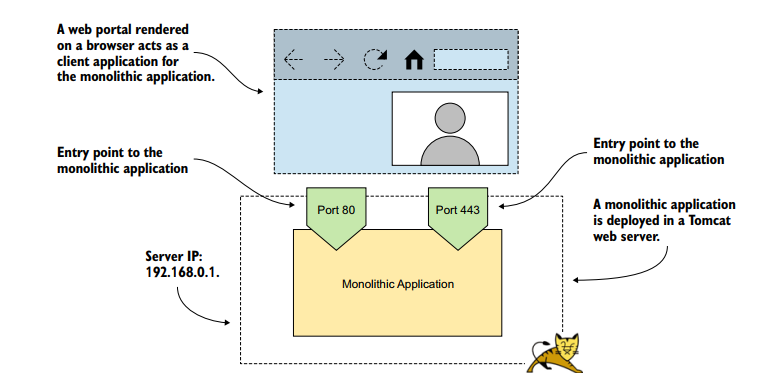
\includegraphics[width=0.7\linewidth]{Pics/monolithic-1}
		\caption{\label{fig:nodes} Ứng dụng monolithich cơ bản.}
		\label{fig:nodes}
	\end{figure}
	\hspace{0.3cm}{Trong hầu hết các ứng dụng nguyên khối, bảo mật được thực thi tập trung và các thành phần riêng lẻ không cần phải lo lắng về việc thực hiện các kiểm tra bổ sung trừ khi có yêu cầu khẩn cấp để
	làm như vậy. Do đó, mô hình bảo mật của ứng dụng nguyên khối đơn giản hơn nhiều so với mô hình bảo mật của ứng dụng được xây dựng trên kiến trúc microservice.}

	\subsection{Nguyên tắc cơ bản trong bảo mật bảo mật microservice}
	\subsubsection{Tính xác thực}
	\hspace{1.0cm}{Xác thực là quá trình xác định bên yêu cầu để bảo vệ hệ thống của bạn chống giả mạo. Bên yêu cầu có thể là một hệ thống (một microservice) hoặc một hệ thống yêu cầu quyền truy cập thay mặt cho người dùng là con người hoặc một hệ thống khác. Tuy nhiên, rất khó có khả năng người dùng là con người sẽ truy cập trực tiếp vào một microservice. Trước khi tạo một thiết kế bảo mật cho một hệ thống nhất định, bạn cần xác định đối tượng. Phương pháp xác thực bạn chọn dựa trên đối tượng.}
	
	\begin{figure}[h]
		\centering
		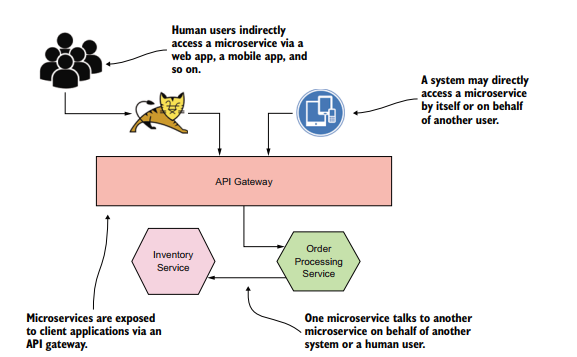
\includegraphics[width=0.7\linewidth]{Pics/authentication}
		\caption{\label{fig:nodes} Các đối tượng xác thực.}
		\label{fig:nodes}
	\end{figure}

	\hspace{0.3cm}{Để xác thực người dùng với một hệ thống (ví dụ: ứng dụng web), ứng dụng có thể yêu cầu tên người dùng và mật khẩu với một yếu tố khác cho xác thực đa yếu tố (MFA). MFA có bắt buộc hay không chủ yếu là do quyết định kinh doanh, dựa trên mức độ quan trọng của tài sản kinh doanh của bạn hoặc mức độ nhạy cảm của dữ liệu bạn muốn chia sẻ với người dùng.}

	\subsubsection{Tính toàn vẹn}
	\hspace{1.0cm}{Khi bạn truyền dữ liệu từ ứng dụng khách của mình sang một vi dịch vụ hoặc từ một vi dịch vụ này sang một vi dịch vụ khác—tùy thuộc vào độ mạnh của kênh liên lạc mà bạn chọn—kẻ xâm nhập có thể chặn liên lạc và thay đổi dữ liệu để có lợi cho chúng. Ví dụ: nếu kênh mang dữ liệu tương ứng với một đơn đặt hàng, thì kẻ xâm nhập có thể thay đổi địa chỉ giao hàng thành địa chỉ của chính họ. Các hệ thống được bảo vệ cho tính toàn vẹn không bỏ qua khả năng này; họ giới thiệu các biện pháp để nếu một tin nhắn bị thay đổi, người nhận có thể phát hiện và loại bỏ yêu cầu.}
	
	\hspace{0.3cm}{Cách phổ biến nhất để bảo vệ tính toàn vẹn của một thông điệp là ký tên vào nó.Mọi dữ liệu truyền qua kênh liên lạc được bảo vệ bằng Bảo mật tầng truyền tải (TLS) đều được bảo vệ toàn vẹn. Nếu chúng ta sử dụng HTTPS để liên lạc giữa các vi dịch vụ (trên thực tế, giao tiếp đó là HTTP qua TLS), thư sẽ được bảo vệ toàn vẹn trong khi truyền.}
	
	\hspace{0.3cm}{Cùng với dữ liệu đang truyền, dữ liệu ở trạng thái nghỉ phải được bảo vệ toàn vẹn. Trong tất cả dữ liệu kinh doanh, các dấu vết kiểm tra quan trọng nhất để kiểm tra tính toàn vẹn. Kẻ xâm nhập có quyền truy cập vào hệ thống sẽ hạnh phúc nếu họ có thể sửa đổi các dấu vết kiểm tra để xóa sạch mọi bằng chứng. Trong quá trình triển khai vi dịch vụ dựa trên container, nhật ký kiểm tra không được lưu giữ ở mỗi nút chạy vi dịch vụ; chúng được xuất bản trong một số loại hệ thống theo dõi phân tán như Jaeger hoặc Zipkin. Chúng ta cần đảm bảo rằng dữ liệu được duy trì trong các hệ thống đó được bảo vệ toàn vẹn.}
	
	\subsubsection{Tính chống chối bỏ}
	\hspace{1.0cm}{Chống chối bỏ là một khía cạnh quan trọng của bảo mật thông tin ngăn cản bạn từ chối bất cứ điều gì bạn đã thực hiện hoặc cam kết. Hãy xem xét một ví dụ thực tế. Khi bạn thuê một căn hộ, bạn đồng ý với các điều khoản và điều kiện với công ty cho thuê.}
	
	\hspace{0.3cm}{Nếu bạn rời khỏi căn hộ trước khi kết thúc hợp đồng thuê, bạn có nghĩa vụ trả tiền thuê cho thời gian còn lại hoặc tìm người thuê khác để thuê lại căn hộ. Tất cả các điều khoản đều có trong hợp đồng cho thuê mà bạn chấp nhận bằng cách ký tên vào đó. Sau khi bạn ký tên, bạn không thể tranh chấp các điều khoản và điều kiện mà bạn đã đồng ý. Đó là điều không thể phủ nhận trong thế giới thực. Nó tạo ra một nghĩa vụ pháp lý. Ngay cả trong thế giới kỹ thuật số, một chữ ký giúp bạn đạt được sự không từ chối; trong trường hợp này, bạn sử dụng chữ ký điện tử.}
	
	\hspace{0.3cm}{Bạn cũng cần đảm bảo rằng bạn ghi lại các giao dịch cùng với dấu thời gian và chữ ký—đồng thời duy trì các bản ghi đó trong một khoảng thời gian đáng kể. Trong trường hợp người khởi xướng tranh chấp giao dịch sau này, bạn sẽ có giao dịch đó trong hồ sơ của mình.}
	
	\subsubsection{Tính sẵn sàng}
	\hspace{1.0cm}{Toàn bộ quan điểm của việc xây dựng bất kỳ loại hệ thống nào là cung cấp cho người dùng. Cứ mỗi phút (hoặc thậm chí là giây) hệ thống ngừng hoạt động, doanh nghiệp của bạn sẽ mất tiền. Amazon đã ngừng hoạt động trong 20 phút vào tháng 3 năm 2016 và tổn thất doanh thu ước tính là 3,75 triệu USD. Vào tháng 1 năm 2017, hơn 170 chuyến bay của Delta Airlines đã bị hủy do hệ thống ngừng hoạt động, dẫn đến thiệt hại ước tính 8,5 triệu USD.}
	
	\hspace{0.3cm}{Không giống như trong các ứng dụng nguyên khối, trong triển khai vi dịch vụ, toàn bộ hệ thống sẽ không ngừng hoạt động nếu phát hiện thấy lỗi trong một thành phần hoặc vi dịch vụ. Chỉ microservice đó sẽ ngừng hoạt động; phần còn lại sẽ có thể hoạt động. Trong tất cả các yếu tố có thể làm hệ thống ngừng hoạt động, bảo mật có vai trò then chốt trong việc giúp hệ thống luôn sẵn sàng cho các bên liên quan hợp pháp của nó. Trong triển khai microservices, với nhiều điểm vào (có thể tiếp xúc với internet), kẻ tấn công có thể thực hiện tấn công từ chối dịch vụ (DoS) hoặc tấn công từ chối dịch vụ phân tán (DDoS) và đánh sập hệ thống.}
	
	\hspace{0.3cm}{Phòng thủ chống lại các cuộc tấn công như vậy có thể được xây dựng trên các cấp độ khác nhau. Ở cấp độ ứng dụng, điều tốt nhất bạn có thể làm là từ chối một tin nhắn (hoặc một yêu cầu) ngay khi bạn thấy rằng nó không hợp pháp. Có kiến trúc bảo mật theo lớp giúp bạn thiết kế từng lớp để xử lý các loại tấn công khác nhau và từ chối kẻ tấn công ở lớp ngoài cùng.}
	
	\pagebreak
	
	\textbf{Kết luận chương 1}
	
	\hspace{1.0cm}{Qua chương một, chúng ta đã tìm hiểu về kubernetes là gì, kiến trúc và cách thức hoạt động của kubernetes. Và tổng quan về microservice, các nguyên tắc để bảo vệ microservice. Nhưng khi mà chúng ta triển khai hệ thống microservice trên kubernetes, chúng ta làm thế nào để có thể bảo mật được các microservice. Nếu như một hệ thống lớn, có hàng trăm đến hàng ngàn microservice, thì liệu chúng ta có thể chỉ cần triển khai bảo mật trên hệ thống mà không cần phải sửa lại tất cả microservice đó không. Điều này là có thể đối với Service Mesh, một trong những công nghệ giúp chúng ta triển khai trên mặt hệ thống giúp bảo mật các ứng dụng microservice. Vậy, service mesh là gì, cách hoạt động của nó như nào, chúng ta sẽ đến với chương 2. Ở chương 2, chúng ta sẽ nói tổng quan về service mesh và công cụ giúp chúng ta triển khai service mesh trên kubernetes là HashiCorp Consul.}
	
	\chapter{Giới thiệu về HashiCorp Consul}
	
	\section{Tổng quát về Service Mesh}
	
	\hspace{1.0cm}{Để bắt đầu hành trình khám phá service mesh, có ba điều mà chúng ta cần phải biết: Service Mesh là gì, cách thức nó hoạt động như nào và tại sao chúng ta lại sử dụng nó.}
	
	\hspace{0.3cm}{Có lẽ, để định nghĩa ngắn gọn service mesh, thì chúng ta có thể hiểu như sau}
	
	\hspace{0.3cm}{Service mesh là lớp kiến trúc hạ tầng mà cho phép bạn kiểm soát giao tiếp mạng của hệ thống của bạn từ một control plan duy nhất.}
	
	\hspace{0.3cm}{Để hiểu hơn về định nghĩa trên, chúng ta cần chia thành các phần sau: }
	
	\hspace{0.3cm}{Thông qua lớp kiến trúc hạ tầng, service mesh không phải là một phần của service, nó được triển khai và vận hành theo một cách độc lập. Vì nó không thể xác định được cụ thể được logic hoạt động của dịch vụ cụ thể, nhưng nó ảnh hưởng đến mọi dịch vụ, nên nó được coi là cơ sở hạ tầng hoặc phần mềm trung gian.}
	
	\hspace{0.3cm}{Dưới đây là hình ảnh của một phần mềm thông thường. Dịch vụ và ứng dụng chạy trên các cơ sở hạ tầng. Service mesh nằmg ở lớp cơ sở hạ tầng đầu tiên với các yêu cầu về lưu trữ, metrics và cơ sở hạ tầng cao cấp khác. Bến dưới đó là Kubernetes, máy ảo hoặc bất kì kiến trúc máy tính nào mà có thể chạy. Bên dưới cùng là phần cứng (bare metal)}
	
	\begin{figure}[h]
		\centering
		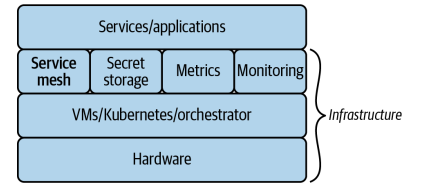
\includegraphics[width=0.7\linewidth]{Pics/software_stack}
		\caption{\label{fig:software_stack} Một khối ứng dụng cụ thể}
		\label{fig:software_stack}
	\end{figure}
	
	\subsection{Phương thức hoạt động của service mesh}
	\hspace{1.0cm}{Service mesh được tạo thành từ các proxy sidecar và control plan.}
	\subsubsection{Proxy Sidecar}
	\hspace{1.0cm}{Proxy là một ứng dụng mà lưu lượng truy cập được định tuyến trên đường đến đích của nó. Các proxy phổ biến mà bạn có thể đã nghe nói đến là NGINX, HAProxy và Envoy. Trong hầu hết các service mesh, tất cả lưu lượng dịch vụ (vào và ra) được định tuyến thông qua một proxy cục bộ dành riêng cho từng phiên bản dịch vụ
	
	\hspace{0.3cm}{Hình bên dưới thể hiện service mesh sẽ như thế nào với 2 đối tượng: frontend và backend. Khí frontend gọi đến backend, proxy cục bộ của frontend sẽ bắt tất cả các yêu cầu được đi ra ngoài. Proxy của frontend sẽ chuyển các yêu cầu đến dịch vụ backend. Khi mà yêu cầu được đưa tới dịch vụ backend, tiếp tục, nó được proxy cục bộ của backend nắm bắt và kiểm tra. Nếu yêu cầu được cho phép, proxy của backend sẽ chuyển tiếp yêu cầu đó đên dịch vụ backend thực tế.}
	\begin{figure}[h]
		\centering
		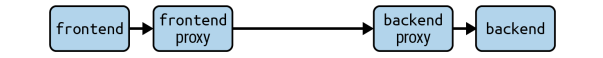
\includegraphics[width=0.7\linewidth]{Pics/proxy}
		\caption{\label{fig:proxy} Hai ứng dụng giao tiếp với nhau thông qua service mesh}
		\label{fig:proxy}
	\end{figure}
	
	\hspace{0.3cm}{Mỗi phiên bản của một dịch vụ phải được triển khai với proxy cục bộ của chính nó. Mẫu triển khai ứng dụng trợ giúp - trong trường hợp này là proxy - cùng với dịch vụ chính được gọi là mẫu sidecar và do đó, proxy cục bộ được gọi là proxy sidecar.}
	
	\hspace{0.3cm}{Proxy Sidecar là một thành phần quan trọng của service mesh vì chúng cho phép kiểm soát lưu lượng dịch vụ mà không cần sửa đổi hoặc triển khai lại các dịch vụ cơ bản. Vì proxy sidecar chạy dưới dạng các quy trình riêng biệt với dịch vụ nên chúng có thể được cấu hình lại mà không ảnh hưởng đến dịch vụ. Ví dụ: proxy sidecar của dịch vụ backend có thể được cấu hình lại để từ chối lưu lượng truy cập từ dịch vụ backend mà không cần thay đổi mã hoặc triển khai lại chính dịch vụ backend.}
	
	\subsubsection{Control Plane}
	\hspace{1.0cm}{Công việc của control plane là quản lý và định cấu hình các proxy sidecar. Như bạn có thể thấy hình bên dưới, control plane là một dịch vụ riêng biệt phải được triển khai riêng; nó không được triển khai như một sidecar. control plane là nơi chứa hầu hết logic phức tạp của service mesh: nó phải theo dõi các dịch vụ bắt đầu và dừng, ký và phân phối chứng chỉ, cấu hình lại proxy, v.v. Bản thân các proxy sidecar tương đối đơn giản: chúng nhận cấu hình từ control plane nêu chi tiết những hành động nào sẽ thực hiện trên lưu lượng truy cập và họ thực hiện những hành động đó.}
	\begin{figure}[h]
		\centering
		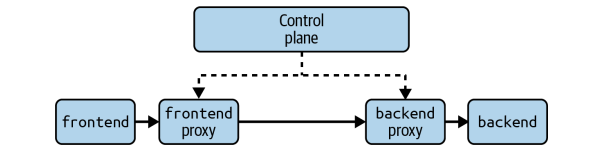
\includegraphics[width=0.7\linewidth]{Pics/control-plane}
		\caption{\label{fig:control-plane} Control plane quản lý các sidecar proxy.}
		\label{fig:control-plane}
	\end{figure}

	\subsection{Các tính năng của Service Mesh}
	\hspace{1.0cm}{Service mesh cung cấp các tính năng trong bốn lĩnh vực: bảo mật, khả năng quan sát, độ tin cậy và kiểm soát lưu lượng. Đề xuất giá trị cơ bản của service mesh là khả năng cung cấp các tính năng này trên mọi dịch vụ và khối lượng công việc mà không cần sửa đổi mã dịch vụ.}
	\subsubsection{Bảo mật}
	\hspace{1.0cm}{Một trong những lý do chính khiến các công ty triển khai service mesh là để bảo mật mạng của họ. Thông thường, điều này có nghĩa là mã hóa lưu lượng giữa tất cả các khối lượng công việc và triển khai xác thực cũng như ủy quyền.}
	
	\hspace{0.3cm}{Giải quyết vấn đề này có thể rất khó khăn trong kiến trúc microservices mà không có service mesh. Yêu cầu mã hóa mọi yêu cầu có nghĩa là cung cấp chứng chỉ Bảo mật tầng vận chuyển (TLS) cho mọi dịch vụ theo cách an toàn và quản lý cơ sở hạ tầng ký chứng chỉ của riêng bạn. Xác thực và ủy quyền mọi yêu cầu có nghĩa là cập nhật và duy trì mã xác thực trong mọi dịch vụ.}
	
	\hspace{0.3cm}{Service mesh giúp công việc này dễ dàng hơn nhiều vì nó có thể cấp chứng chỉ và định cấu hình proxy sidecar để mã hóa lưu lượng và thực hiện ủy quyền - tất cả mà không có bất kỳ thay đổi nào đối với các dịch vụ cơ bản}
	
\end{document}